%
% $RCSfile$
%
% Copyright (c) 2005-2006. Christian Heller. All rights reserved.
%
% Permission is granted to copy, distribute and/or modify this document
% under the terms of the GNU Free Documentation License, Version 1.1 or
% any later version published by the Free Software Foundation; with no
% Invariant Sections, with no Front-Cover Texts and with no Back-Cover
% Texts. A copy of the license is included in the section entitled
% "GNU Free Documentation License".
%
% http://www.cybop.net
% - Cybernetics Oriented Programming -
%
% http://www.resmedicinae.org
% - Information in Medicine -
%
% Version: $Revision$ $Date$ $Author$
% Authors: Christian Heller <christian.heller@tuxtax.de>
%

\subsection{Modelling Mistakes}
\label{modelling_mistakes_heading}

Most modern software is not written directly in a machine language but designed
in form of higher-level models instead. These allow to speed up application
development and help avoiding errors. \emph{Object Oriented Programming} (OOP),
for example, uses design concepts like the \emph{Class} owning \emph{Attributes}
and \emph{Methods}. Yet does this kind of modelling create abstractions that
reflect concepts of the real world completely and correctly?

\begin{figure}[ht]
    \begin{center}
        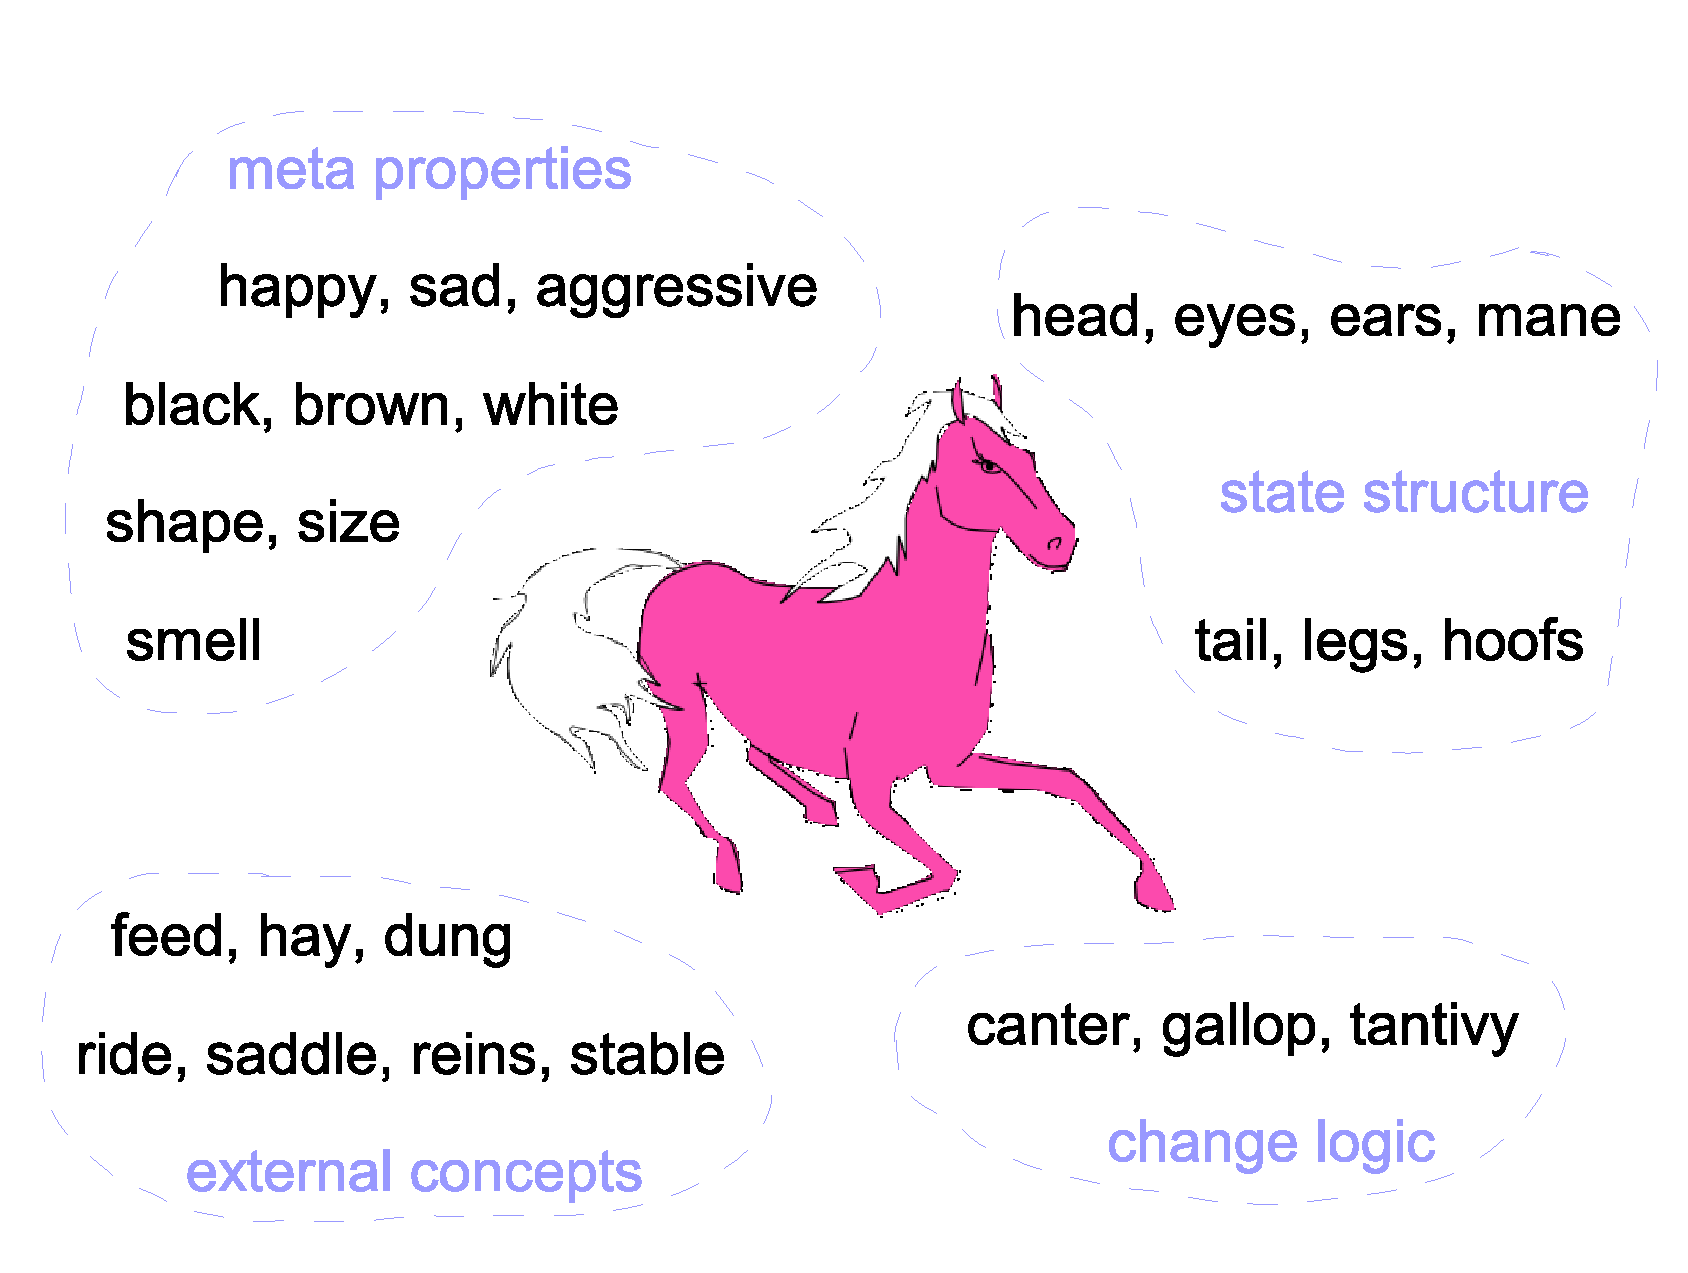
\includegraphics[scale=0.2]{vector/horse.eps}
        \caption{Concept of a Horse}
        \label{horse_figure}
    \end{center}
\end{figure}

The model of a \emph{Horse} shall serve as example to investigate this further.
Figure \ref{horse_figure} shows a number of terms commonly used to create a
model of a horse. Most importantly, there are structural observations
describing the horse as concept consisting of parts like \emph{Head},
\emph{Legs} or \emph{Hoofs}. Secondly, there are properties like the horse's
\emph{Colour}, \emph{Shape} or \emph{Size}. Thirdly, there are terms describing
a horse's actions like its \emph{Movement} or \emph{Eating}, that change a
horse's position and/ or state. Finally, there are a number of terms like
\emph{Hay} or \emph{Saddle} associating concepts related to the horse.

One might suggest to model properties like the position, size or colour of a
horse's leg as \emph{Part} of that leg. In fact, this is how classical
programming approaches its solutions. In OOP, one would probably use a class
representing the leg and an attribute standing for the leg's colour. However,
when following the modelling principles of human thinking (see
\cite{heller2004}), this is \emph{not} correct!

It is true that in everyday language, one tends to say \textit{A horse leg
\emph{has a} colour.} Unfortunately, this leads to the wrong assumption that a
leg were made of a colour. But this is not the case. A leg does not
\emph{consist} of a colour in the hierarchical meaning of a whole consisting of
parts. The colour is rather property information \emph{about} the leg. It seems
there is no correct expression in natural (English) language stating the
property of something. The \emph{IS-A} verbalisation is used to express that
the leg belongs to a special category of items, for example: \textit{A leg is a
body element.} The \emph{HAS-A} formulation is used to express that a leg as
whole consists of smaller parts, for example: \textit{A leg has a knee and it
has a hoof.} But which formulation expresses a property? Well, perhaps it would
be best to say: \textit{A leg IS-OF a colour.}

The CYBOP knowledge schema described later in this article (section
\ref{knowledge_schema_heading}) distinguishes structural whole-part- from meta
information. Actions (like the gallop of a horse) causing change in the model
or its environment are called \emph{Logic}, since they follow certain rules.
